\section{Budowa i analiza diagramu przepływu danych - Data Flow Diagram }
% \textit{Ma na celu określenie przepływu danych (wejścia, wyjścia, operacje, przechowywanie) oraz
% elementów sterowania tym przepływem, co może być pomocne dla tworzenia aplikacji.
% Specyfikacja danych wejściowych i wyjściowych.}
\begin{figure}[!htp]
  \centering
  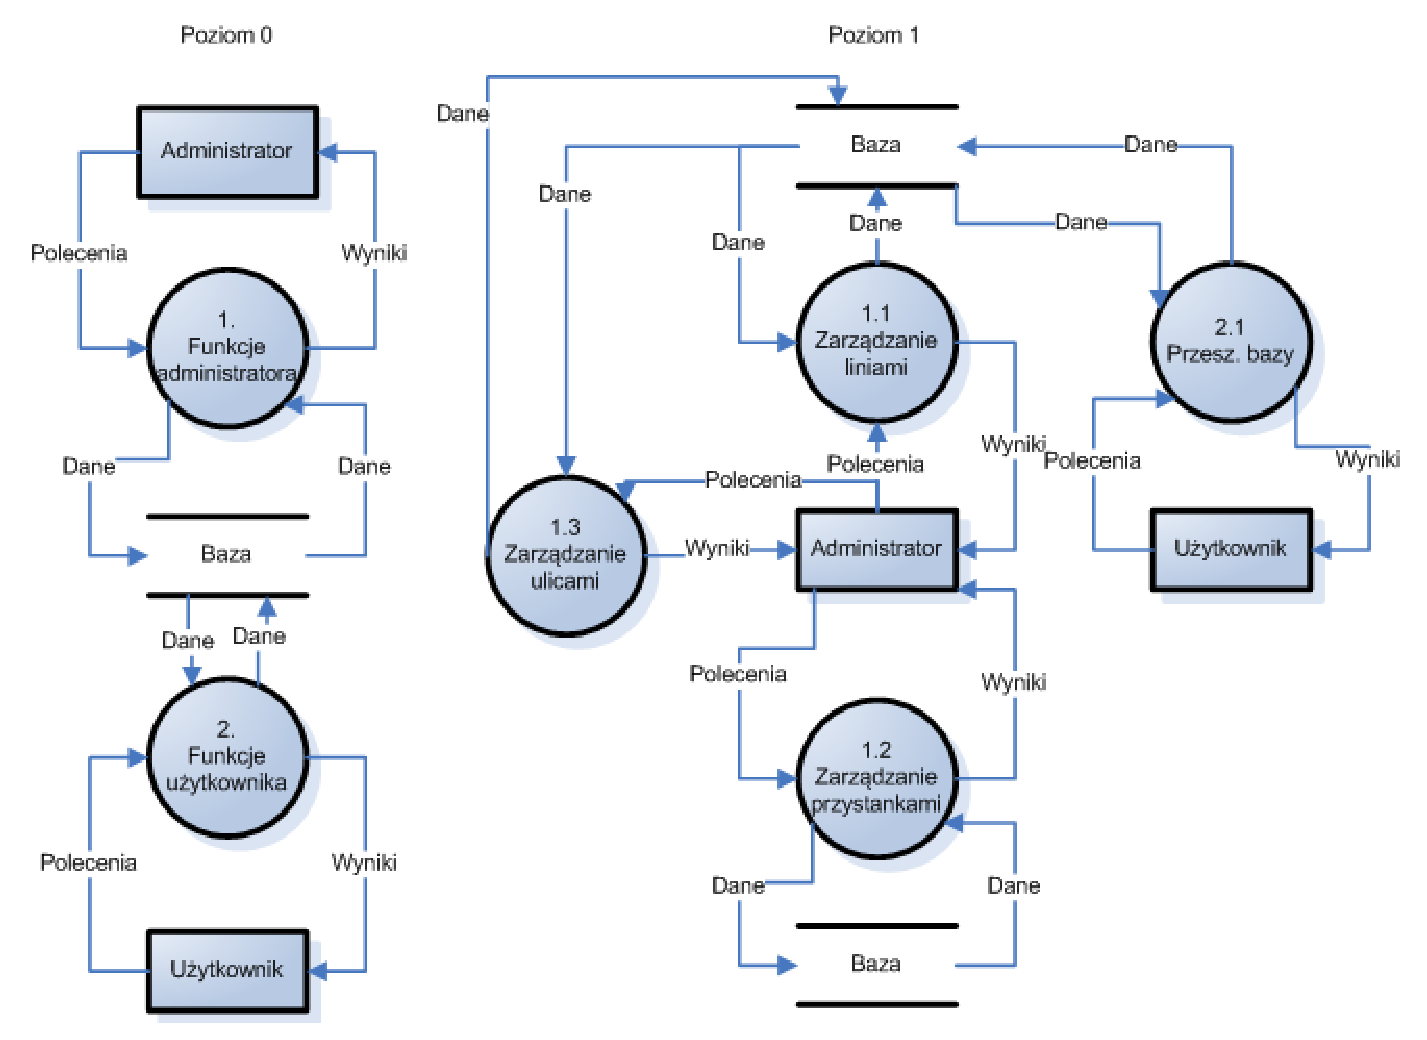
\includegraphics[width=0.8\textwidth]{./img/schema_a.eps}
  \caption{Diagram DFD}
  \label{fig:scr3a}
\end{figure}
\begin{figure}[!htp]
  \centering
  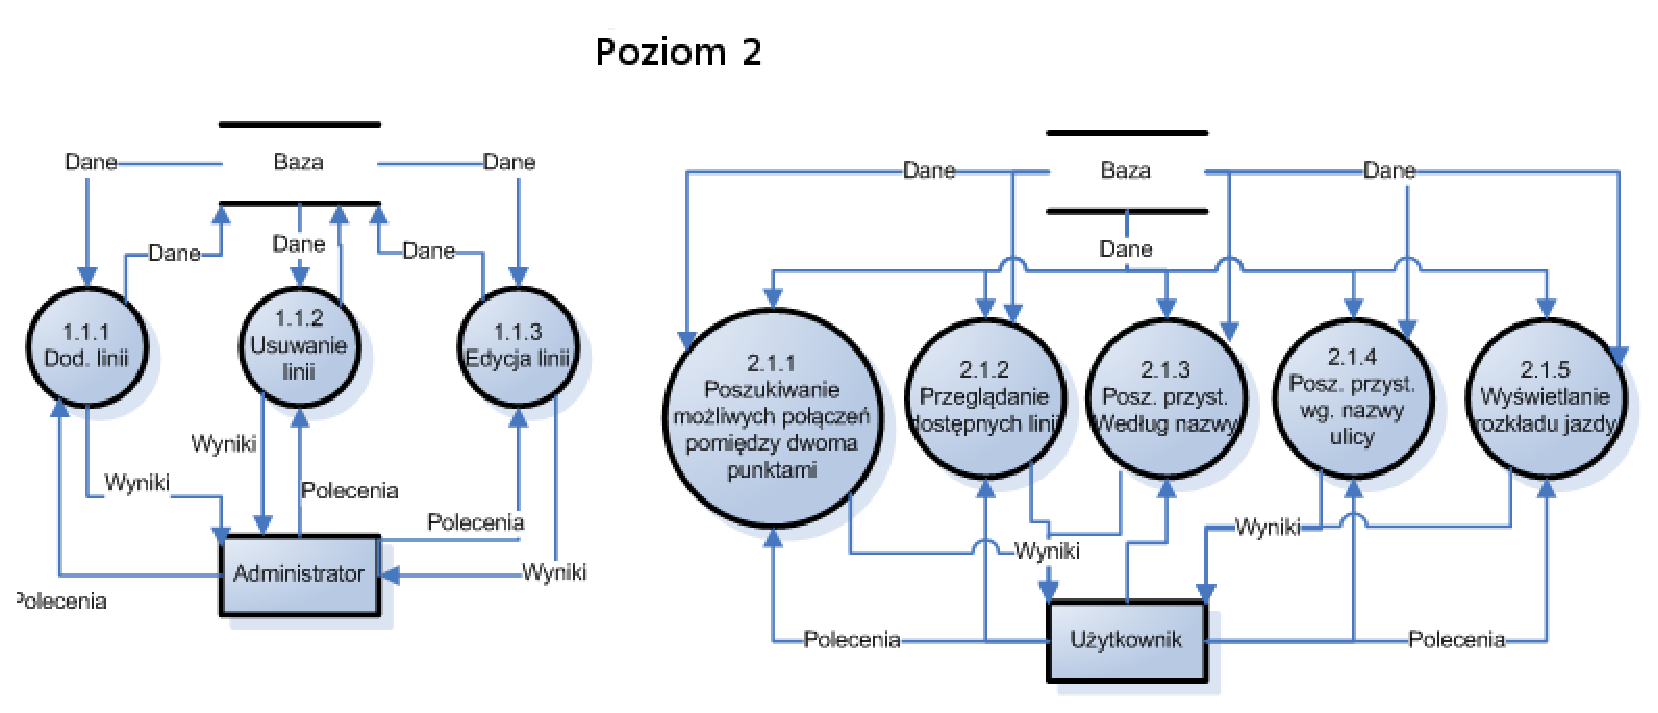
\includegraphics[width=0.8\textwidth]{./img/schema_b.eps}
  \caption{Diagram DFD}
  \label{fig:scr3b}
\end{figure}
